\chapter{Qu'et-ce qu'une fonction}
Une fonction est un objet mathématique qui associe une valeur à une autre. On peut se représenter l'effet d'une fonction par une boîte noire. Une valeur est entrée dans la boîte noire et une autre valeur en ressort. Une fonction décrit le comportement de cette boîte; elle décrit les opérations que subiront la valeur d'entrée pour être transformée en valeur de sortie. Si on connaît la fonction on peut déterminer toutes les valeurs de sortie. 
%mettre illusatration boite noire 
%mettre exemples fonctions
Une fonction a un domaine de départ et un domaine d'arrivée. Le domaine de départ est l'ensemble des valeurs que peut prendre la fonction en argument: l'ensemble des valeurs qu'"accepte la boîte noire".

Le domaine d'arrivée est l'ensemble des valeurs que la fonction/la boîte noire peut retourner.

Chaque valeur du domaine correspond à une seule valeur du domaine d'arrivée, %mettre contre-exemple: cercel
ceci n'est pas forcément réciproque. Si c'est le cas on dit que la fonction est \textbf{bijective}.%mettre diagramme sagittal + exemple

%nsérer déf injective et surjective
\section{Représentation d'une fonction}
Dans le cadre de ce livre, nous allons uniquement considérer des fonctions à un variable. Dans ce cas on observe l'évolution de la fonction, généralement dénotée $f(x)$, en fonction de $x$, il s'agit donc de couples de valeurs, $(x,f(x))$. En mathématiques, il est courant de représenter ces couples dans un graphique.

Un graphique est composée de deux droites.
Une droite horizontale: l'\textbf{abscisse}, souvent dénoté comme l'axe des $x$ et une droite verticale l'\textbf{ordonnée} également appelée axe des $y$.

L'abscisse représente la première valeur du couple et l'ordonnée la deuxième. $y$ est donc associée à $f(x)$ pour la représentation.
\begin{figure}[h!]
  \caption{A picture of a gull.}
  \centering
    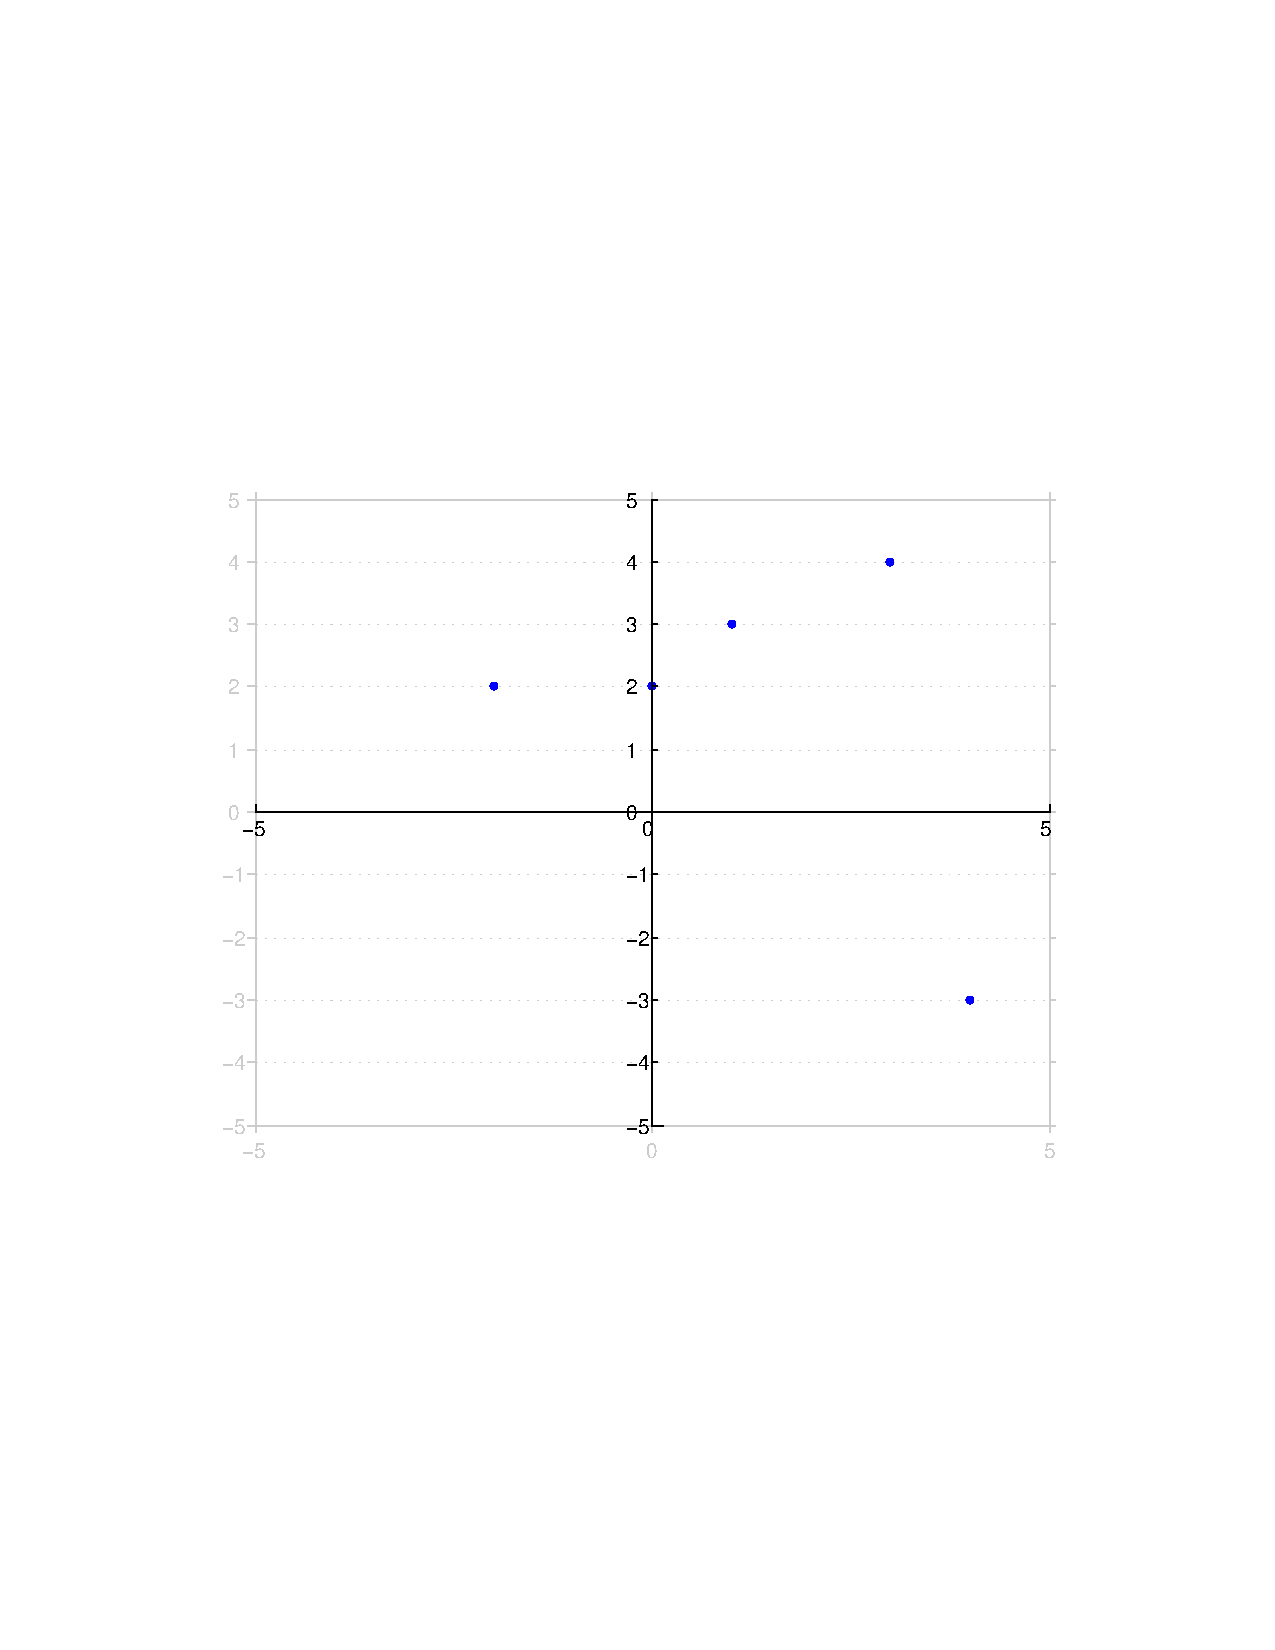
\includegraphics[width=0.5\textwidth]{matlab/es}
\end{figure}


L'intersection